\begin{figure*}
  \centering
  \begin{subfigure}[t]{0.43\linewidth}
    \centering
  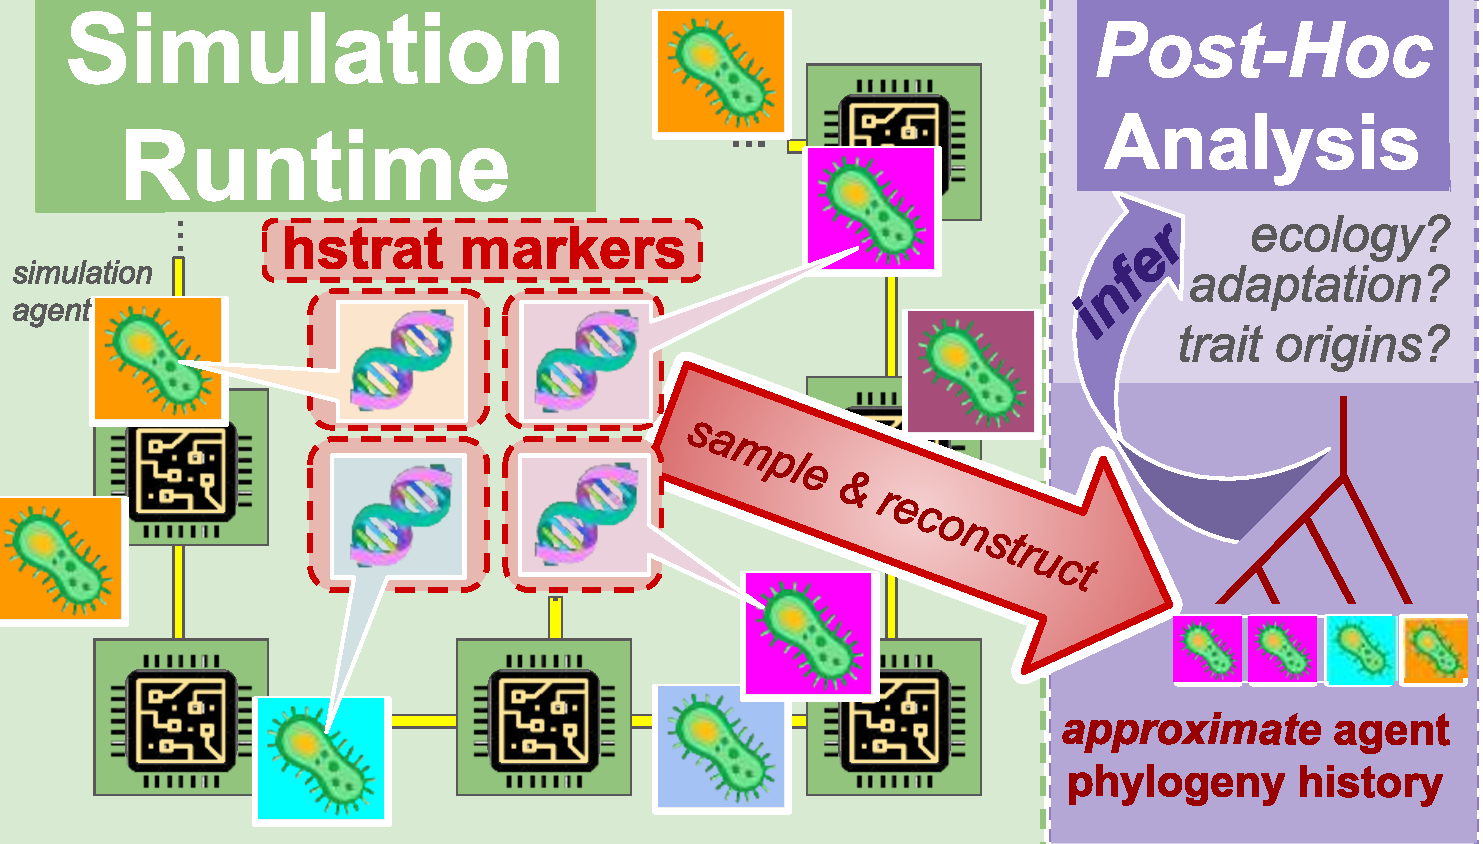
\includegraphics[width=\linewidth]{binder-wse-sketches/tex-access-proposal/img/runtime-posthoc-schematic}
    \caption{%
    Proposed agent-based evolutionary simulation and observation framework, using HStrat markers to estimate phylogenetic history, thereby, infer evolutionary dynamics.
    }
    \label{fig:runtime-posthoc-schematic}
  \end{subfigure}
  \hspace{0.07\linewidth}
  \begin{subfigure}[t]{0.43\linewidth}
    \centering
  \includegraphics[width=\linewidth]{binder-wse-sketches/tex-access-proposal/img/async-ga-schematic}
    \caption{Schematic overview of asynchronous island model evolutionary algorithm implementation.}
    \label{fig:async-ga-schematic}
  \end{subfigure}

\caption{%
\textbf{Summary of proposed experimental framework.}
Subfigure \ref{fig:runtime-posthoc-schematic} overviews proposed distributed simluation strategy.
Subfigure \ref{fig:async-ga-schematic} summarizes asynchronous population exchange strategy used to simulate evolving populations on Cerebras Wafer Scale Engine hardware.
}
\label{fig:schematic}

\end{figure*}
